%% go to the website http://en.wikibooks.org/wiki/LaTeX For Help 
\documentclass[11.5pt]{article}
%Math Related Packages
\usepackage{mathtools}
\usepackage{amsmath}
\usepackage{amsfonts}
\usepackage{amssymb}
\usepackage{relsize}
% Pseudocode Packages
%\usepackage{algorithm}
%\usepackage{algpseudocode}
\usepackage[colorinlistoftodos]{todonotes}
% Automata/Graph Packages
\usepackage{tikz}
\usepackage{pgf}
\usetikzlibrary{arrows,automata}
\usepackage[latin1]{inputenc}
\usetikzlibrary{automata,positioning}
%%%Formatting Options for Pages
%\usepackage[a4paper,left=2cm,right=2cm]{geometry} %Change Margins
\usepackage[colorlinks=true, allcolors=blue]{hyperref} % adds hyperlinks
\usepackage{listings}
\usepackage{multicol}
\usepackage{perpage}
\MakePerPage{footnote}
%%%Graphics Packages and Caption Tools
\usepackage{graphicx}
\usepackage{fullpage}
\newcounter{Figure} 
\setcounter{Figure}{1}
%\usepackage{slashbox}
\usepackage{ulem}
\usepackage{csvsimple}
%%%Colors Package with Custom Defined Colors
\usepackage{color}
\usepackage{colortbl}
\definecolor{codegreen}{rgb}{0,0.6,.2}
\definecolor{codegray}{rgb}{0.5,0.5,0.5}
\definecolor{codepurple}{rgb}{0.58,0,0.82}
%%Custom Functions and Commands
\newcommand\indentFour{\indent\indent\indent\indent}
\newcommand\indentThree{\indent\indent\indent}
\newcommand\indentTwo{\indent\indent}
\newcommand\tab{\ \ \ }
\newcommand\proof{\setcounter{equation}{0}\hfill\fbox{\rule{.02in}{0pt}\rule[0ex]{0pt}{.5ex}}}

%%Math Commands
\newcommand{\Lbra}{\left\langle}
\newcommand{\Rbra}{\right|}
\newcommand{\Rket}{\right\rangle}
\newcommand{\Lket}{\left|}
\newcommand{\bra}[1]{\Lbra #1 \Rbra}
\newcommand{\ket}[1]{\Lket #1 \Rket}
\newcommand{\braket}[1]{\Lbra #1 \Rket}
\newcommand{\Exists}{\ \exists \ }
\newcommand{\Forall}{\ \forall \ }
\newcommand{\abs}[1]{\left| #1 \right|}
\newcommand{\Frac}[2]{\left(\frac{#1}{#2}\right)}
\newcommand{\Mat}[1]{\left[\begin{matrix} #1 \end{matrix}\right]}
\newcommand{\vhi}{\varphi}
\newcommand{\R}{\ \mathbb{R}}
\newcommand{\C}{\ \mathbb{C}}
\newcommand{\N}{\ \mathbb{N}}
\newcommand{\Z}{\ \mathbb{Z}}
\newcommand{\I}{\ \mathbb{R/Q}}
\newcommand{\x}{\mathrm{x}}
\newcommand{\mbf}[1]{\mathbf{#1}}
\newcommand{\Dpart}[2]{\frac{\partial #1}{\partial #2}}
\DeclarePairedDelimiter{\ceil}{\lceil}{\rceil}
\newcommand{\U}{\underline}
%Numbering
\newcounter{graphics}
\newcounter{tables}
\renewcommand{\abstractname}{Abstract}

\begin{document}
\title{Deep Learning for Knowledge Graph Completion}
\author{Nick Joodi$^\dagger$, Kevin Jesse$^\dagger$, Cesar Bartolo-Perez$^\dagger$, Doug Sherman$^\dagger$\\
	{\small\textit{$^\dagger$ University of California - Davis}}
} 
\date{November 30th, 2017}
\maketitle
\rule{\textwidth}{1pt}

\begin{abstract}

\end{abstract}

\tableofcontents

\section{Introduction}
\paragraph{} With the advent of Google's knowledge Graph, Wikidata, Freebase, and many others, the representation of data in the form of a knowledge base or ontology is affecting our lives everyday. Data in this format has been used to power advanced reasoning systems, chat bots, and in general, Artificial Intelligence. However, these knowledge bases are many times incomplete. To counter this, knowledge graph completion has been researched extensively over recent years. 

\paragraph{} Knowledge graph completion is the act of inferring new "facts" over an existing knowledge base. To represent a knowledge base as a knowledge graph, one can treat the concepts/entities/objects within the knowledge base as nodes and the relations/predicates between these concepts as edges. After applying this conversion, the knowledge will be a large interlinking web of objects relating to one another, I.e a knowledge graph. A fact, in this case, is an instance in a knowledge graph where two objects are linked by a predicate. The common notation for this fact, or triplet, is the following:  (s,p,o) where s and o are nodes in the graph, and p is the edge. Given two objects, knowledge graph completion gives us the ability to predict, with a measurable certainty, whether or not a triplet exists.

\paragraph{} There have been a variety of techniques used to perform knowledge graph completion: translation, logically based, and deep learning techniques. This paper will focus on applying deep learning to this problem domain. The two neural network architectures that we will apply are the neural tensor network and the multi layered perceptron. 

\paragraph{} The neural tensor network, introduced by Socher et. al, has been shown to provide intriguing results. Since its emergence, it has been used as a baseline to evaluate the newer architectures in the field. This model incorporates a tensor layer in addition to the standard components of a neural network, to express the relationship between two entities. More over, this work also incorporated the useful approach in representing each entity as a composition of its word embeddings. They've shown, that using pretrained word embeddings enhances the performance of the overall model.

\paragraph{}Conversely, a more standard, simpler approach to this problem is the use of a multi layered perceptron. [citation] has shown comparable results to the more computationally intensive neural tensor network.

\paragraph{}We took these two architectures and applied them to a subset of the Wikidata knowledge base. More specifically, we focused on the familial relationship between humans. To the best of our knowledge, knowledge graph completion has not been done over this subset of the Wikidata knowledge base.

\paragraph{}This paper has the following outline. In the next section, we will cover the methods and assumptions that we used to build and trained our models, followed by a section describing our results, then a discussion, and finally a conclusion to summarize as well as state potential future work.

\section{Methods}
\subsection{Architecture}
\subsubsection{Multilayered Perceptron Model (MLP}
\paragraph{}We implimented a Multiyaler Perceptron (MLP) model using the RSNNS package following the Stuttgart Neural Network Simulator\cite{RSNNS}. Figure \ref{MLPArch} shows a general look at the architecture for our MLP design. We tested a few variations of the MLP model to determine the suitable parameters for our dataset; including a variable number of layers, activation functions, and nodes per layer. Moreover, we tuned the hyperparameters such as the learning rate and momentum term for backpropagation. We will reference Figure \ref{MLPArch} as we discuss the effects of the different architectures. 


\begin{figure}[h!]
 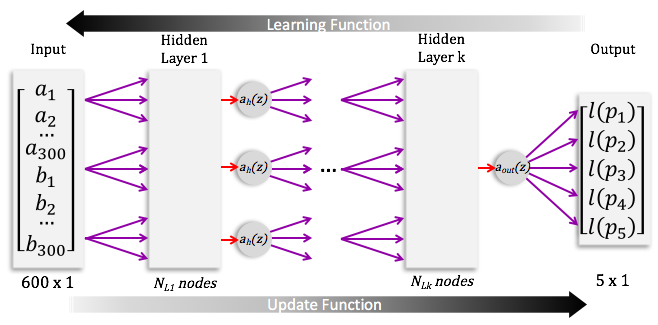
\includegraphics[width=1\textwidth]{report_mlp/GenArchitecture.png}
  \caption{\small A general look at the Neural Network architecture used for a MLP model with $k$ hidden layers with $N_{L_i}$ nodes for the $i$th layer, a common activation function $a_h(z)$ for each layer, and a final output activation function $a_{out}(z)$. The way that these activations propagate through the network is defined by the update function (e.g. simultaneously or sequentially), and the error propagates back according to the learning function. We have 600 features from our input, 1 for each dimension of both entity embeddings, and we are predicting the true/false value of our 5 output predicates. Note that $l(p_1)$ is the likelihood that the predicate $p_1$ is true.  }
  \label{MLPArch}
\end{figure}


\paragraph{}
Much consideration was made in regards to the architecture of the MLP model. These include decisions on how the weights will propagate through the model, how error is propagated back from predictions, and how the first initialization of the weights is determined. A list of these parameters is given below
\begin{center}
\begin{tabular}{|ll|}
\hline
\textbf{Function  }& \textbf{Description } \\%& Examples & Our Choice\\
\hline
\textbf{Activation} & The function applied after each hidden layer. \\%& $\tanh$, Logistic, RELU & Logistic/Sigmoid \\
\textbf{Initialization} & How parameters of the Neural Network are initialized before training. \\%& Random, All 0 or 1, All Positive & Random\\
\textbf{Learning} & How error is propagated from predicted outputs. \\%& Std Back Propagation, BackProp with Momentum &  BackProp with Momentum\\
\textbf{Update} & How the activation functions are propagated through the network. \\%& Simultaneously, In-Order & In-Order (Topologically)\\
\hline
\end{tabular}
\end{center}

We tested different combinations of functions to best suit knowledge graph completion, and ultimately decided on using a sigmoid activation function, random initializations,  backpropagation with momentum to speed up convergence, and a toplogical (in order) method for forward propagation. The sigmoid activation function was chosen for each hidden layer of our MLP architecture because it demonstrated the highest, and most reliable, accuracy than other options such as $\tanh$ or ReLU.

\paragraph{} More importantly, we tested many different architecture sizes. The size includes how many hidden layers, and the size of these hidden layers. To determine this, 
many architectures were tested and the error per iteration for both training and testing sets along with test set ROC curves, were considered in the final determination. These tests are illustrated in the Results section of this report.

\subsubsection{Neural Tensor Network (NTN)}
\paragraph{}  We implemented the Neural Tensor Network (NTN) using TensorFlow 1.3. The architecture was based on [citation]. The scoring function is as follows:

\begin{equation}
g(e_1,R,e_2)  = u_R^Tf \bigg( e_1^TW_R^{[1:k]}e_2 + V_R + V_R 
\bigg[ \begin{matrix}  e_1 \\ e_2  \end{matrix} \bigg] + b_R \bigg)
\end{equation}

\paragraph{}  Where  $ W_R^{[1:k]} \in \R^ {d * d * k} $, $ V_R \in \R^ {k * 2d} $, $ b_R \in \R^ {k } $, and  $ u \in \R^ {k } $. d is the size of the embedding and k is the number of slices in the tensor. Each relation $R$ has its own network with the above aforementioned parameters. The model leverages this tensor parameter, $ W_R^{[1:k]} $ to relate the two entity inputs in a multiplicative manner. This is in contrast to the more standard neural network (an MLP leveraging just parameters $ V,u,b $) where the entities are simply concatenated to one another. See Figure \ref{ntn_arch.png} for a visualization. Additionally, all networks share a parameter matrix, $E \in \R^{w*d} $, where w is the number of unique words contained in the knowledge graph, and d representing the embedding size. This parameter is used to determine the entity embeddings as discussed in section 2.2.

\paragraph{}  To train the model, the contrastive max margin loss was minimized:


\begin{equation}
J(\Omega)  = \sum_{i=1}^{N} \sum_{c=1}^{C} max \bigg(0,1 - g\bigg( T^(i) \bigg) +  g\bigg( T_c^(i) \bigg)   \bigg)
\end{equation}

\paragraph{}  Where $ \Omega $ represents the training parameters, $N$ is the number of training samples, $C$ is the corruption size, and $T$ represents the inputs of the triplet to the scoring function. At every training step, each positive triplet, $T$, is duplicated $C$ times. The score for that triplet and then also a corrupted triplet is determined using the neural tensor network scoring function. The corrupted triplet is created by removing either the head entity or tail entity from the triplet with a randomly chosen entity in the entity set. The objective is to increase the margin between the correct and corrupted triplet. We used AdaGrad optimization to train the model. Robert Socher et al. used L-BFGS optimization; however, this type of optimization does not come with the standard distribution of TensorFlow 1.3.

 \begin{figure}[h!]
\centerline { 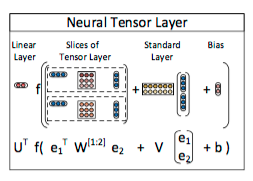
\includegraphics[width=.5\textwidth]{report_ntn/ntn_arch.png}}
  \caption{The architecture of the Neural Tensor Network. A layer of the tensor is indicated by a dashed rectangle}
  \label{ntn_arch.png}
\end{figure}

\subsection{Data Curation}


\paragraph{} The dataset we considered was queried from the WikiData, a free opensource knowledge base that acts as the central storage device for its sister projects including Wikipedia, Wikivoyage, and Wikisource \cite{Wikidata}. Wikidata offers a SPARQL type queries for obtaining data on a variety of sources. We queried data regarding the lineage of many famous people in history including: Frederik, Crown Prince of Denmark, George Windsor, Earl of St Andrews, and Shigeko Higashikuni. The relations we considered were if one person, or entity, was the Father, Mother, Spouse, Sibling, or Child of another. See Figure \ref{query} for an example of the query we used to obtain our dataset. 


\begin{figure}[h!]
 \lstinputlisting[language=Matlab]{code/SparqlQuery.txt}
 \caption{\small SPARQL query used to obtain our raw data from Wikidata}
 \label{query}
\end{figure}


\paragraph{} The raw data is a table of values that lists each person and their Father, Mother, spouse, sibling, and child; leaving an entry empty if unknown. We processed this table into positive triplets of the form \texttt{(Q193752, P25, Q229279, 1)} where \texttt{Q193752} and \texttt{Q229279} are a unique encoding of the target and related entities respectively, \texttt{P25} represents one of the relations, or predictes, and \texttt{1} indicates that this statement is true. In english this triplet implies that \texttt{Q229279} is the \texttt{P25} of \texttt{Q193752}. These positive facts represent all the data we can pull directly from the knowledge graphs. However, to increase the robustness of our data, we can create negative facts as well. For example, since we know that Cleopatra VII Philopator, the last active pharaoh of Ptolemaic Egypt, was the daughter of Ptolemy XII Auletes, we can conclude she was not the daughter of Richard Nixon. Thus we can extend our data to contain these negative triplets of the form \texttt{(Q1,P1,Q2,-1)}. In all, we were able to produce 37395 positive triplets and 37391 negative triplets from our raw data. 

\paragraph{} In an effor to exploit the uniqueness in the names for each of our entities, we used word embeddings of each of the words in a name to generate entity embeddings. We used the Fasttext model to generate word embeddings from semantic anaylsis across Wikipedia. Fasttext is a library that represents words as bags of character $n$-grams for fast and efficient classification \cite{BojanowskiGJM16,JoulinGBM16}. Thus, we used Fasttext to obtain $300\times 1$ word embeddings of each of the unique words found in all of our entitie's names. For example, the name "Charles Stuart, 1st Earl of Lennox", we found an 300 dimensional embedding vector for Charles, Stuart, 1st, Earl, of, Lennox. Once each of the words had embeddings, we could construct entity embeddings for each of our entities. The method we used for this was to aggregate the word embeddings by taking the mean across each of the words within an entity name. For the MLP model, if Fasttext could not produce a valid embedding for a given word, then that word was ignored. Moreover, if an entity consisted entirely of unknown words, then that entity was thrown out. We did this to preserve the integrity of our input data because in the standard MLP model we would not be training these embeddings. However, for more complex models, another suitable technique is to randomize the embeddings for these entities, or all entities, to guarantee a more representative dataset. Overall, only about 6.4\% of the entities had no suitable embedding. 

\subsubsection{Data staging (MLP)}
\paragraph{}  Once we encoded each entity with their embedding we produced a dataset where each row contains the numeric representation of a triplet. Hence, for a triplet given by \texttt{(EntityA,Pred2,EntityB,1)}, where the embedding for \texttt{EntityA} and \texttt{EntityB }is $[a_1,a_2,\cdots,a_{300}]^T$ and $[b_1,b_2,\cdots,b_{300}]^T$ respectively, the associated row in our data set is given by
$$ \Mat{a_1,a_2,a_3,\cdots,a_{300},b_1,b_2,\cdots,b_{300},0,1,0,0,0} $$
where the last 5 columns represents the truth values for each of the 5 predicates (Father, Mother, Spouse, Sibling, Child).

\subsubsection{Data staging (NTN)}
\paragraph{}  One of the learned parameters for the NTN is the word embeddings. Therefore, before every training step, the entity embeddings had to be recalculated. The word embeddings were represented as a n x d matrix, where n represents the number of unique words across all the entities, and d representing the size of the embedding. Each row index mapped to a unique word. The entity embeddings were then determined by taking the average of the word embeddings that were contained in that entity. The resulting entity embeddings were stored in an n x d matrix, where n was the number of entities across the knowledge graph, and d was the size of the embeddings.

\paragraph{} The training, development, and testing sets contained the triplets, representing a fact in the knowledge graph. The data sets were loaded into an n size matrix, where n was the number of triplets, and each row of the matrix contained the index mapping to the corresponding entity, predicate, as well as the truth value for that triplet. From there, the matrix was grouped into subset matrices corresponding to each predicate.

\section{Results}
\subsection{MLP}
In order to prevent overfitting in our model, we have compared our model with 100 and 50 interations (Figure \ref{50_100_128.png}). We can notice that under 100 iterations, the training error drops to a weigthed SSE of almost 500. However, our testing error, start increasing after 30 itearions aproximately. From this results, we can infer that we have reached an overfitting in our model and a smaller number of iterations are enougth. In that sense, we have run our model with 50 iterations, avoiding the increase in the SSE.\par
 

\begin{figure}[h!]
 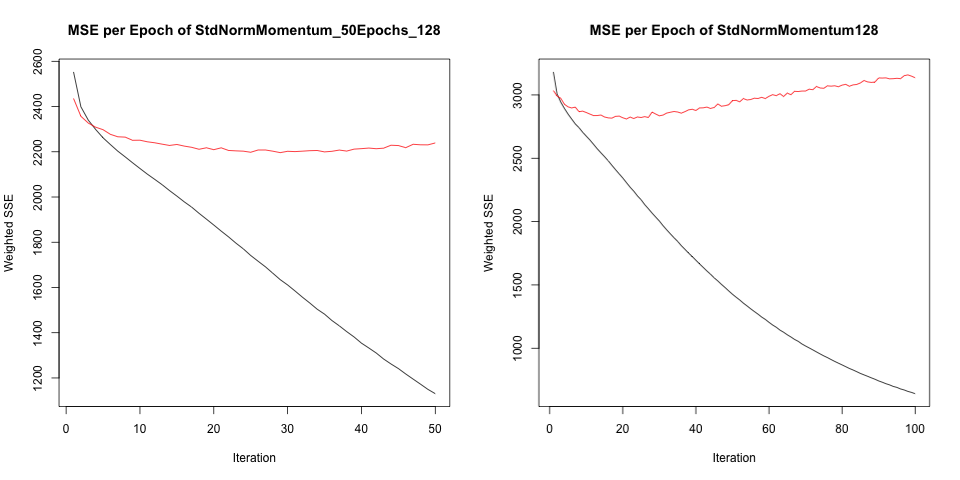
\includegraphics[width=1\textwidth]{report_mlp/50_100_128.png}
  \caption{\small MSE at different iterations. The structure presents a single hidden layer with 128 nodes}
  \label{50_100_128.png}
\end{figure}


In a second running of the model, we have added a new hidden layer  with different number of nodes (16,64 and 128). Before 50 iterations, adding nodes to the second hidden layer, reduce the error in our model. However, after 50 iteration, the higher number of nodes, increase rapidly the overfitting  of the model. \par 


\begin{figure}[h!]
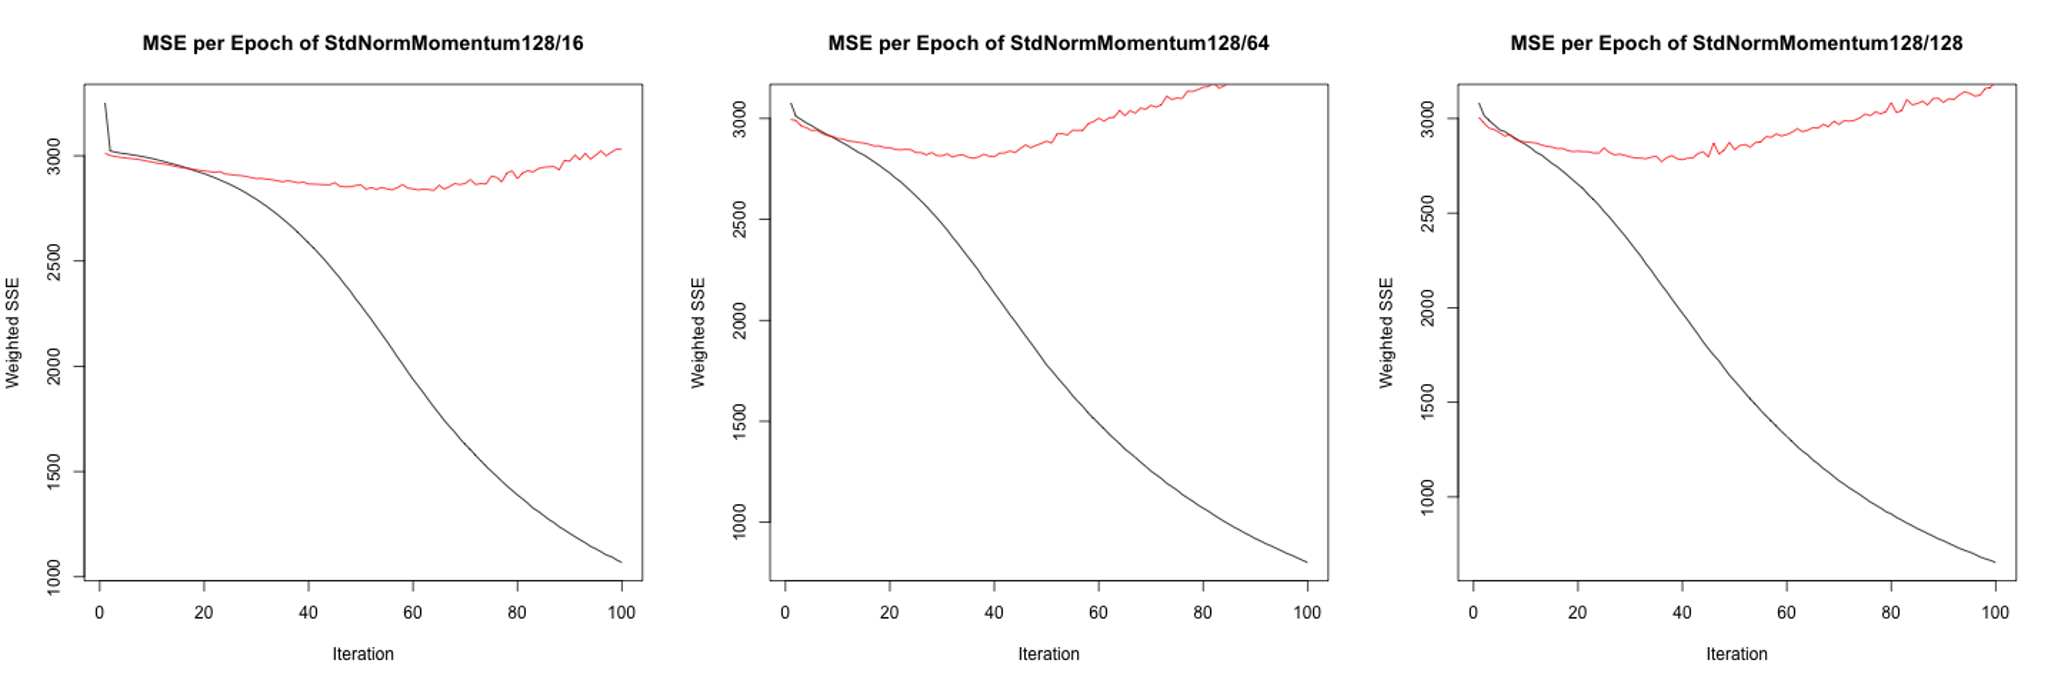
\includegraphics[width=1\textwidth]{report_mlp/128-16_64_128.png}
  \caption{\small MSE for A NN with two hidden layers with different nodes at second hidden layer.}
\label{128-16_64_128.png}
\end{figure}

In  a following set of tests, we compared different Neural Networks structures, increasing the number of hidden layers (hidden layers/nodes: 128, 128/16 and 128/128/16).  Figure \ref{128-16_64_128.png} shows that for the model with three hidden layers the training error is not decreasing considerably before 40 iteration. Suddently, the SSE in this NN structure drops abruptaly. The training error, shows that the error keep increasing at that range of iterations. This beahvior, can be attributed to an overfitting in our model. \par

Ths trend described above is similar for two hidden layers. For the case of just one hidden layer with 128 nodes, the error does not drop abruptly for the training set but we can see an increase in the error for after 30 iterations aproximately. \par 

These results, make us suggest that only one hidden layer is enough for our MLP model, since there is not a big improvement in the reduction of error with more layers added and with the benefit of less computational resources are required.
This decision is confirmed comparing their ROC curves for each NN structure.
 
\begin{figure}[h!]
  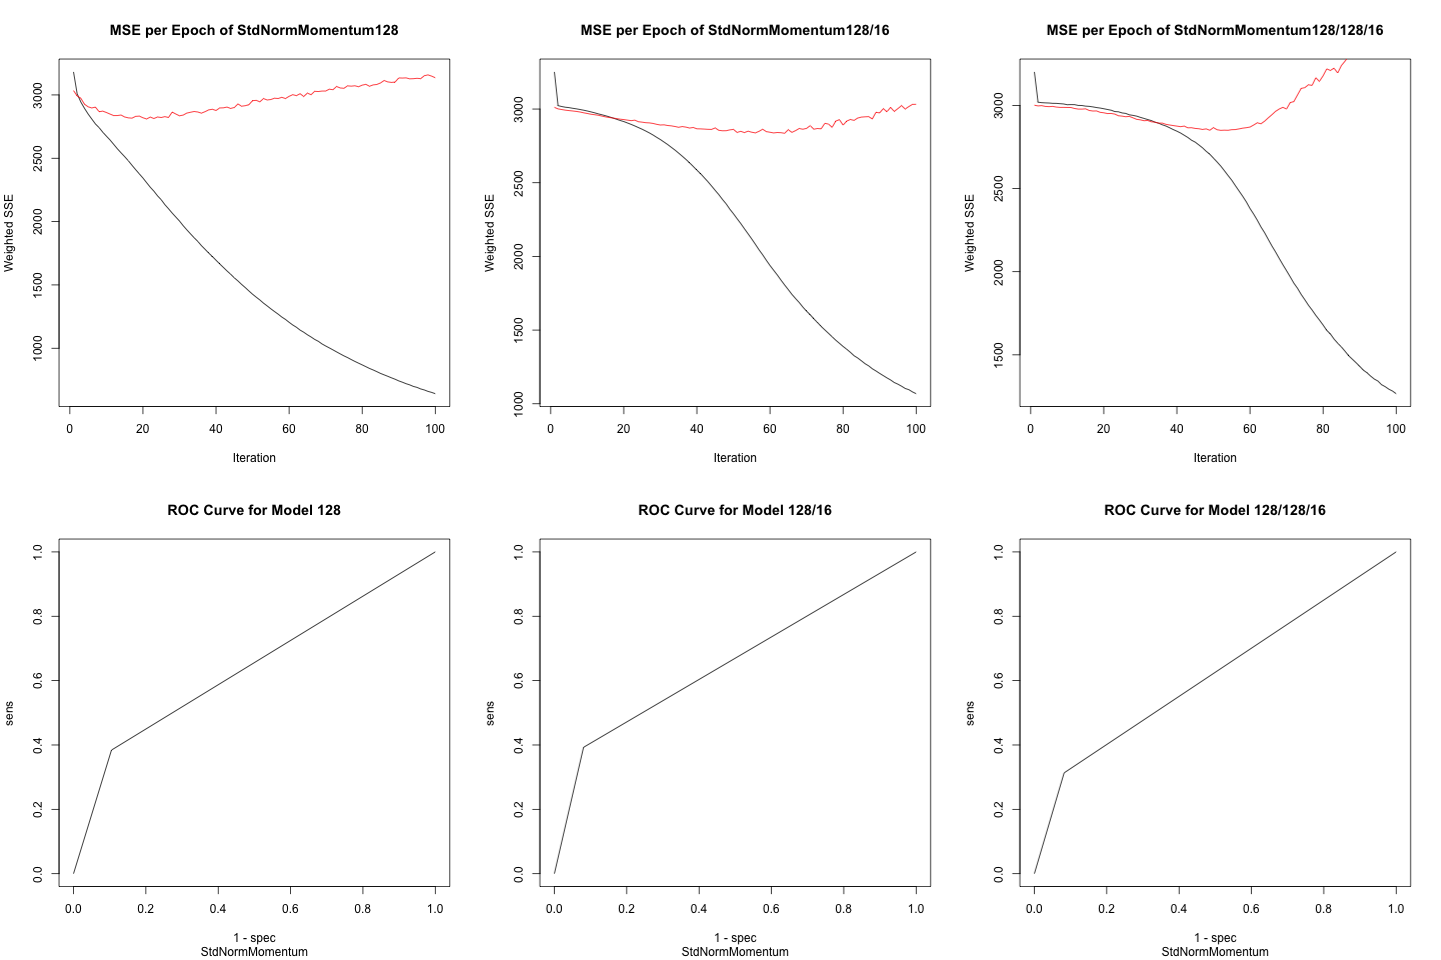
\includegraphics[width=1\textwidth]{report_mlp/different_layers_MSE_ROC.png}
    \caption{\small MSE and ROC curves for different levels of hidden layers}
    \label{different_layers_MSE_ROC.png}
\end{figure}

\subsection{NTN}
\paragraph{} When training the NTN, the embedding size was set to 300 to be inline with the FastText pretrained embedding size, corruption size set to 10, tensor layer slice size set to 3, L2 regularization set to .0001, and the number of iterations set to 1500 with a batch size of 10000. We cross validated over a development set to determine the threshold for each relation network. 

\paragraph{} We first trained the model on randomly initialized word embeddings . We then cross validated on our testing set. See Figure \ref{performanceRandomNtn.jpg} for detailed statistics. The loss began to converge at about 800. The ROC curve showed a respectable 0.906 AUC. With the exception of the spouse classification, all accuracies were 80\% or higher, with the overall accuracy being 88\%. With respect to the MLP implementation, these are very respectable results.

\paragraph{} Also of interest, is the noticeable clustering of the word embeddings after training the model. See Figure \ref{random_init_tsne.jpg}. Both tSNE plots show the same 500 word embeddings before and after training. These groupings of the word embeddings that are occurring indicate a learned semantic relationship with one another.

\paragraph{} We also trained the model over pretrained word embeddings and evaluated it over the same testing set. See Figure \ref{pretrain_perf.jpg} for detailed statistics. One will quickly notice that the pretrained word embedding model actually performed worse than the randomly initialized word embedding model. This more than likely occurred due to the large portion of words represented in the entities were missing from the pretrained FastText embedding model. We only saw a total of 1735 words from the FastText pretrained model that matched the over 6035 unique words found in the entities. We had to drop 2305 entities since there was no word contained in the respective entity that was found in the pretrained model. Additionally, given that we dropped a word from the entity if we did not have a match in our pretrained model, we had over 50\% of the entities have at least one other duplicated embedding value with respect to another entity. Although this is not an ideal testing condition for the nueral tensor network over pretrained word embeddings, we still found it intriguing that the results were actually worse than the randomly initialized word embedding model. This further argues, in line with Socher et al., that the initialization technique performed on the word embeddings plays a powerful role in the performance of the model.


\begin{figure}[h!]
\centerline{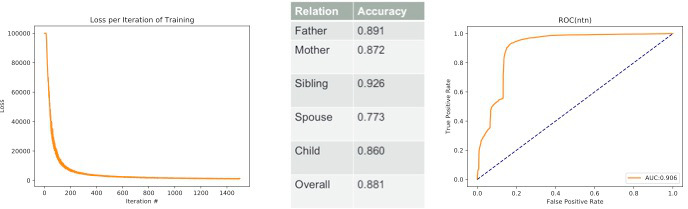
\includegraphics[width=1\textwidth]{report_ntn/performanceRandomNtn.jpg}}
  \caption{From left to right:Contrastive Max margin loss with respect to iteration for random initialization of word embeddings, Accuracy for each relation network for the ideal threshold, the overall ROC curve}
\label{performanceRandomNtn.jpg}
\end{figure}

\begin{figure}[h!]
\centerline{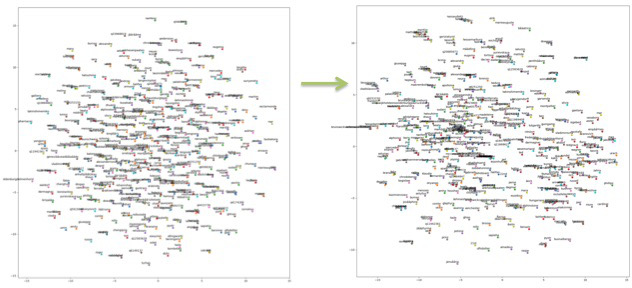
\includegraphics[width=1\textwidth]{report_ntn/random_init_tsne.jpg}}
  \caption{The left tSNE plot visualizes the word embeddings at the start of training. The right tSNE plot visualizes the word embeddings at the end of training}
\label{random_init_tsne.jpg}
\end{figure}

\begin{figure}[h!]
\centerline{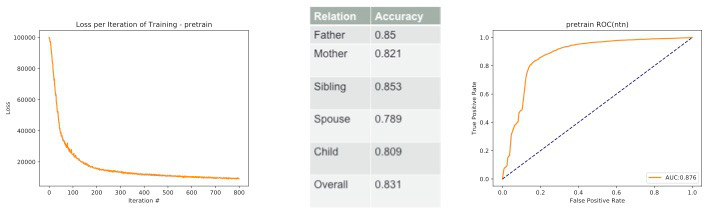
\includegraphics[width=1\textwidth]{report_ntn/pretrain_perf.jpg}}
  \caption{From left to right:Contrastive Max margin loss with respect to iteration for pretrained initialization of word embeddings, Accuracy for each relation network for the ideal threshold, the overall ROC curve. Note: There was a significant portion of words that were missing from the pretrained FastText embedding model the more than likely impacted the results}
\label{pretrain_perf.jpg}
\end{figure}

\section{Discussion}

\bibliographystyle{ieeetr}
\bibliography{bib}{}

\end{document}